\documentclass[UTF-8,twoside,cs4size]{ctexart}
\usepackage{amsmath}
\usepackage{amssymb}
\usepackage{geometry}
\usepackage{setspace}
\usepackage{xeCJK}
\usepackage{ulem}
\usepackage{pstricks}
\usepackage{pstricks-add}
\usepackage{bm}
\usepackage{mathtools}
\usepackage{breqn}
\usepackage{mathrsfs}
\usepackage{esint}
\usepackage{textcomp}
\usepackage{upgreek}
\usepackage{pifont}
\usepackage{tikz}
\usepackage{circuitikz}
\usepackage{caption}
\usepackage{xcolor}
\usepackage{tabularx}
\usepackage{array}
\usepackage{pgfplots}
\usepackage{multirow}

\newcolumntype{Y}{>{\centering\arraybackslash}X}
\geometry{a4paper,centering,top=0.75cm,bottom=2.54cm,left=2cm,right=2cm}
\pagestyle{plain}
\captionsetup{font=small}

\CTEXsetup[name={,.}]{section}
\CTEXsetup[format={\raggedright\bfseries\noindent\Large}]{section}
\CTEXsetup[format={\raggedright\bfseries\quad\large}]{subsection}
\CTEXsetup[format={\raggedright\bfseries\qquad}]{subsubsection}

\setstretch{1.5}

\setCJKfamilyfont{boldsong}[AutoFakeBold = {2.17}]{SimSun}
\newcommand*{\boldsong}{\CJKfamily{boldsong}}
\DeclareMathOperator\dif{d\!}
\newcommand*{\me}{\mathop{}\!\mathrm{e}}
\newcommand*{\tab}{\indent}

\begin{document}
	\begin{flushright}
		\zihao{2}{分组号:3-07}
	\end{flushright}
	
	\noindent{\zihao{-2}\boldsong\bfseries 《\,\, 基\,\, 础\,\, 物\,\, 理\,\, 实\,\, 验\,\, 》\,\, 实\,\, 验\,\, 报\,\, 告\,\, }
	
	\noindent\textit{实验名称\uline{\quad\qquad\qquad\qquad 光栅光谱仪\qquad\,\qquad\qquad\qquad\qquad\qquad}指导教师\uline{\qquad\,\,\,常亚男\,\,\,\qquad}}
	
	\noindent\textit{姓\qquad 名\uline{\,\,\, 桂庭辉\,\,\,}\,学号\uline{\,\,\,{\upshape2019K8009929019}\,\,\,}\,专\qquad 业\uline{\,\,\,计算机科学与技术\,\,\,}\,班级\uline{\,\,\,\upshape{03}\,\,\,}\,座号\uline{\,\,\,\upshape{6}\,\,\,}}
	
	\noindent\textit{实验日期\uline{\,\,{\upshape 2020}\,\,}年\uline{\,\,{\upshape 11}\,\,}月\uline{\,\,{\upshape18}\,\,}日\,\,实验地点\uline{\,\,\,教学楼{\upshape713}\,\,\,}调课/补课\uline{\,\,\,$ \square $是\,\,\,}成绩评定\uline{\,\,\,\quad\qquad\qquad}}
	
	\begin{table}[h]
		\centering
		\psset{linewidth=2pt}
		\begin{pspicture}(-1,-0.1)(1,0.1)
		\psline(-9,0)(9,0)
		\end{pspicture}
	\end{table}

	\section{实验目的}
	1.了解光栅光谱仪的结构原理;
	
	2.掌握一种标定光栅光谱仪的方法;
	
	3.学会用光栅光谱仪测绘物质的光吸收谱;
	
	4.掌握测定未知光波波长的一种方法;
	
	5.测量氢原子的巴尔末系发射光谱;
	
	6.基于CCD采集的多通道测量模式。
		
	\section{实验器材}
	WGD-8型组合式多功能光谱仪,溴钨灯,汞灯,氢灯,钠灯,样品。
		
	\section{实验原理}
	\subsection{光栅光谱仪}
	光栅光谱仪是用光栅作为色散元件的分光仪器,可用于产生单色光、光源的光谱分析或材料的光谱特性测量等,是目前应用最广泛的一种光谱仪器。本实验使用的Czerny-Turner型光栅光谱仪是一种色散型光栅光谱仪。经由仪器内的光路,最终我们在出射狭缝处得到的是某一波长的单射光,通过转动其光栅,最终可获得不同波长的单色光。
	
	色散型光栅光谱仪有四个基本的光学性能指标,它们分别是色散率、分辨本领、光谱工作范围与聚光本领。它们与光栅仪所使用的光学元器件质量,如反射镜与光栅的性能指标、狭缝宽度和外部配套系统有关,一般认为光栅性能指标和狭缝宽度是其中最重要的因素。
	
	(1)色散率:色散型光栅光谱仪的色散率可分为角色散率和线色散率。角色散率$ D_\theta $的定义是波长差$ \Delta\lambda=\lambda_1-\lambda_2 $的光经光栅衍射后同级衍射光的衍射角差$ \Delta\theta=\theta_1-\theta_2 $与$ \Delta\lambda $的比值,即
	\[D_\theta=\frac{\Delta\theta}{\Delta\lambda}\]
	根据光栅方程可得到波长$ \lambda $的光经光栅衍射后的第$ k $级衍射的$ D_\theta $值为
	\[D_\theta=\frac{k}{d\cos\theta}\]
	其中$ d $为光栅常数,其倒数$ \frac1d $表示每毫米所含光栅刻线数目,常叫做光栅空间频率。为获得大的角色散率,应采用光栅空间频率大的光栅为色散元件的光栅光谱仪。
	
	线色散率$ D_l $是描述两条光谱线在出射面分开的程度,其定义是两条谱线$ \lambda $和$ \lambda+\Delta\lambda $被分开的限度$ l $
	\[D_l=\frac{l_1}{\Delta\lambda}\]
	若光栅光谱仪内部凹面反射镜$ \mathrm M_3 $的焦距为$ f $,对经过校验的正常工作光谱仪,其角色散率与线色散率有关系为:
	\[D_l\approx fD_\theta\]
	故而应用长焦距的凹面反射镜能提高光谱仪的色散率。
	
	(2)分辨本领:用光谱仪分辨本领标志该仪器能分辨开紧挨着的两条光谱线的本领。其定义为刚可被分开的两条光谱线的平均波长$ \bar\lambda $与它们波长差$ \Delta\lambda $的比值,即
	\[R=\frac{\bar\lambda}{\Delta\lambda}\]
	根据瑞利判据,若一条光谱线强度极大点正好与另一条光谱线极小点重合,则这两条谱线能被分开。光栅光谱仪的光栅分辨本领为$ R'=kN $,其中$ k $为衍射级,$ N $为光栅使用面积的刻线总数目。光谱仪的分辨本领还与被测量的谱线强度分布线型、狭缝宽度、外光路系统等因素有关,但简化讨论时往往用$ R' $近似表示$ R $。
	
	(3)波长工作范围:光栅光谱仪工作波长范围主要由光栅和探测器件决定,根据光栅方程,由于入射角和衍射角不能大于$ 90^\circ $,故而光栅测量的长波限$ \lambda_M<2d $。给定光栅后,该光栅光谱仪工作波长范围基本固定。若只从光栅空间频率看光栅光谱仪工作波长范围,大致有下表关系:
	\begin{table}[h]
		\centering
		\renewcommand\arraystretch{1.5}
		\begin{tabularx}{\textwidth}{cYYYYY}
			\hline
			$ \frac1d(\text{线}\cdot\mathrm{mm}^{-1}) $ & $1\sim50$ & $ 50\sim 100 $ & $ 200\sim 600 $ & $ 600\sim1200 $ & $ 1200\sim 1300 $\\
			\hline
			工作波长范围 &\textit{远红外区}&\textit{中红外区}&\textit{近红外区}&\textit{可见区}&\textit{真空紫外区}\\
			\hline
		\end{tabularx}
		\caption{光栅空间频率与光栅光谱仪工作波长范围的对应关系}
	\end{table}

	实验使用闪耀光栅把入射的大部分能量集中到某一特定的衍射角度,以减弱无用的零级光强而增强被测光谱区内强度。此特定衍射角对应的波长称为闪耀波长$ \lambda_b $,其光强可达到入射光强的80\%,闪耀光栅的使用为$ \frac23\lambda_b-2\lambda_b $,其实际上决定光栅的波长范围。
	
	(4)聚光本领:聚光本领反映光谱仪对入射光的利用率。显然出射光强与仪器的透过率成正比,减少各光学元件的损耗可提高聚光本领,此外增大收集光束的张角也可提高聚光本领。由于C-T型光谱仪采用的是对称光路,系统的孔径光阑有凹面镜的直径$ D $确定,因而聚光的立体角正比于$ \left(\frac Df\right)^2 $,其中$ f $为凹面镜的焦距。
	
	\subsection{介质的光吸收谱}
	如有一束波长为$ \lambda $的平行光波垂直通过一各向同性均匀介质,经过$ d_x $薄层后,强度由$ I_0 $减为$ I_0-\dif I $,可认为衰减的百分比$ \frac{\dif I}{I_0} $与通过的距离$ d_x $成正比,即
	\begin{equation}\label{3-2-1}
		\frac{\dif I(\lambda)}{I_0(\lambda)}=\alpha d_x
	\end{equation}
	起哄$ \alpha(\lambda) $是介质的吸收系数,其为波长的函数,单位为$ \mathrm{cm}^{-1} $。测量时只能测量厚度为$ d $的样品前、后的光强,故而对式(\ref{3-2-1})积分,可得
	\begin{equation}\label{3-2-2}
		I(\lambda)=I_0(\lambda)\me^{-\alpha(\lambda)d}
	\end{equation}
	其中$ I_0(\lambda) $为入射光强,$ I(\lambda) $为出射光强。此式也成为朗伯定律。
	
	\begin{figure}[h]
		\centering
		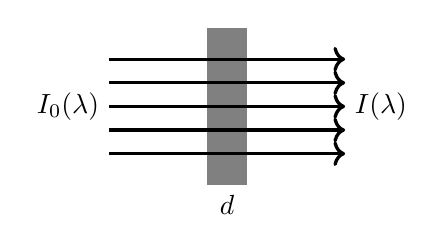
\begin{tikzpicture}
			\fill [gray] (-0.25,-1) rectangle (0.25,1);
			\draw [very thick,->] (-1.5,0)--(1.5,0);
			\draw [very thick,->] (-1.5,0.3)--(1.5,0.3);
			\draw [very thick,->] (-1.5,0.6)--(1.5,0.6);
			\draw [very thick,->] (-1.5,-0.3)--(1.5,-0.3);
			\draw [very thick,->] (-1.5,-0.6)--(1.5,-0.6);
			\node [left] at(-1.5,0) {$ I_0(\lambda) $};
			\node [right] at(1.5,0) {$ I(\lambda) $};
			\node [below] at(0,-1) {$ d $};
		\end{tikzpicture}
		\caption{介质的光吸收示意图}
	\end{figure}

	由上式可得
	\begin{equation}\label{3-2-3}
		\alpha=\frac1d\ln\left(\frac{I_0}{I}\right)=\frac1d\ln\left(\frac1T\right)
	\end{equation}
	其中$ T=\frac{I}{I_0} $为样品的光透过率。
	
	由式(\ref{3-2-3})可用实验数据计算出光吸收系数$ \alpha $随波长$ \lambda $变化的关系曲线,即为$ \alpha-\lambda $曲线,叫做介质的光吸收谱。
	
	一般情况下光吸收系数$ \alpha $与物质的浓度$ C $成正比,即
	\begin{equation}\label{3-2-4}
		\alpha=kC
	\end{equation}
	其中$ k $是单位浓度的吸收系数。将式(\ref{3-2-4})代入式(\ref{3-2-2})可得
	\begin{equation}\label{3-2-5}
		I=I_0\me^{-kCd}
	\end{equation}
	此式即为比尔定律。比尔定律要求物质的吸收系数与浓度无关,也不受周围其他分子的影响。故而在浓度较低时比尔定律正确,而浓度较高时比尔定律失效。但朗伯定律始终成立。
	
	通过率的负对数称为吸光度$ A $,也称为光密度或消光度:
	\[A=-\lg T=\lg\left(\frac1T\right)=\lg\left(\frac{I}{I_0}\right)\]
	由式(\ref{3-2-5})可知,在比尔定律成立时,吸光度$ A $与浓度$ C $成正比。
	
	\subsection{氢原子光谱}
	原子光谱是研究原子能级结构的重要手段,而氢原子(此处指氕)中仅有一个质子和一个电子,是一个简单的二体系统。以氢原子为基础推演出来的基本物理理论也容易用简单的实验来核对,对氢原子光谱的研究极大地推动了量子力学早期的发展。
	
	本实验中观察氢原子光谱中的可见光部分,即巴尔末系的光谱。
	
	\begin{figure}[h]
		\centering
		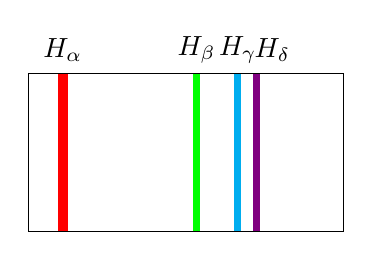
\begin{tikzpicture}
			\draw [red,line width=3.6pt] (-6.56279,1)--(-6.56279,-1);
			\draw [green,line width=2.72pt] (-4.86133,1)--(-4.86133,-1);
			\draw [cyan,line width=2.42pt] (-4.34046,1)--(-4.34046,-1);
			\draw [violet,line width=2.32pt] (-4.10173,1)--(-4.10173,-1);
			\draw (-3,-1) rectangle (-7,1);
			\node at(-6.56279,1.3) {$ H_\alpha $};
			\node at(-4.86133,1.3) {$ H_\beta $};
			\node at(-4.34046,1.3) {$ H_\gamma $};
			\node at(-3.9,1.3) {$ H_\delta $};
		\end{tikzpicture}
		
		\renewcommand\arraystretch{1.5}
		\begin{tabular}{|c|c|c|c|c|}
			\hline
			\textbf{谱线} & $ H_\alpha $ & $ H_\beta $ & $ H_\gamma $ & $ H_\delta $\\
			\hline
			\textbf{波长(nm)} & 656.279 & 486.133 & 434.046 & 410.173\\
			\hline
			\textbf{颜色} & 红 & 深绿 & 青 & 紫\\
			\hline
			$ \bm{\delta\lambda(\mathrm{nm})} $ & 0.181 & 0.136 & 0.121 & 0.116\\
			\hline
		\end{tabular}
		\caption{氢原子的巴尔末系荧光谱示意图及相应的谱线}
	\end{figure}

	氢原子的巴尔末系能级为
	\begin{align*}
		\lambda&=B\frac{n^2}{n^2-4}\qquad n=3,4,5,\cdots\\
		\bar\nu&=\frac1\lambda=R_H\left(\frac{1}{2^2}-\frac{1}{n^2}\right)
	\end{align*}
	
	\section{实验内容}
	\subsection*{·注意事项}
	1.实验中影响光谱强度的主要三个可调节因素:
	
	\tab\tab \textit{光电倍增管电压:$ 300-500\,\mathrm V $即可,不能超过$ 500\,\mathrm V $};
	
	\tab\tab \textit{光源位置:利用软件定点功能,寻找光源最适合的位置};
	
	\tab\tab \textit{入射狭缝宽度适宜:$ 0.02-0.1\,\mathrm{mm} $左右(根据光源情况作适当调整)}。
	
	2.所有光源在实际测量前应尽量预热3-5分钟。氢灯以及Hg/Na灯使用寿命短,做完实验后,需尽快关闭电源,注意安全。
	
	3.在下一个实验开始前,注意选择寄存器保存当前数据。
	
	4.频繁切换CCD与光电倍增管模式容易造成死机,需及时保存数据,并合理安排实验步骤。
	
	5.实验结束后,关闭电源前需将所有倍增电压/电流倍数旋至零位。
	\subsection{CCD功能演示(Hg/Na灯)}
	在光谱仪的CCD模式下,先检索波长,若使用蓝色的Hg灯,则将波长检索到400\,nm;若使用黄色的Na灯,则将波长检索至589.3\,nm。检索后都可观察到几条谱线。在实时显示命令下观察谱线,并改变狭缝宽度以观察谱线的变化。
	
	\subsection{校准单色仪的波长及测量光源的全谱(Hg/Na灯)}
	\subsubsection{校准单色仪的波长}
	由于种种原因,仪器显示的波长值与实际的波长值有一定的偏差,因而在使用前需对单色仪进行校准。具体做法是使用一个或多个能发射线状光谱线的光源,用其已经波长的谱线作为谱线对仪器进行校准。
	
	本次实验中将光谱仪调节至光电倍增管模式,将Hg/Na灯对齐入射狭缝,调节光电倍增管电压至300-500\,V,与计算机上使用相应软件在能量模式下单程采集相应光的谱线,利用自动寻峰功能得到所测得的谱线波长,与已知的标准Hg/Na灯谱线对照,利用波长修正功能适当调整峰值位置。
	
	\textit{已知的$ \mathrm{Hg} $灯谱线为:$ 404.66\,\mathrm{nm},\;435.84\,\mathrm{nm},\;546.07\,\mathrm{nm} $}.
	
	\textit{已知的$ \mathrm{Na} $灯谱线为:$ 589.0\,\mathrm{nm},\;589.6\,\mathrm{nm} $}.
	
	\subsubsection{测量Hg/Na灯全谱}
	将光源尽可能放置得离入射狭缝最近,然后测量全谱。具体指令为在能量模式下已测得的谱线进行自动寻峰,在峰值位置处定点调整光源摆放位置,使得峰值不过高也不过低,调整完成后检波至初始位置,再次进行单程。测量完成后保存全谱,计算每个中心波长的半高全宽值。
	
	\textit{测量$ \mathrm{Hg} $灯所用全谱范围:$ 400\sim600\,\mathrm{nm} $,间距$ 0.1\,\mathrm{nm} $}.
	
	\textit{测量$ \mathrm{Na} $灯所用全谱范围:$ 500\sim700\,\mathrm{nm} $,间距$ 0.1\,\mathrm{nm} $}.
	
	\subsection{测量氢原子光谱}
	在光谱范围$ 400\sim670\,\mathrm{nm} $,取间距为$ 0.02\sim0.04\,\mathrm{nm} $,以上个实验中测全谱的方式测得氢灯光谱。
	
	观察氢原子的巴尔末系光谱,理解原子的能级结构,计算里德堡常数$ R_H $,并进行误差分析,绘制氢原子能级图。
	
	\subsection{测量样品的透过率}
	接通溴钨灯光源,控制溴钨灯光源电流增益$ <1.5\,\mathrm{A} $,在基线模式下,取光谱范围$ 400\sim800\,\mathrm{nm} $,间距为$ 0.1\,\mathrm{nm} $测量溴钨灯自身谱线(即基线)。
	
	分别放入黑/黄/红/蓝/绿色滤波片,在透过率模式下以同样的范围与间距测滤波片透过率,绘制透光率谱图、吸收谱,分别计算吸收系数。
	
	\subsection{测量未知白光光源光谱}
	取用手机闪光灯、LED灯等光源,极可能放置得离入射狭缝最近,在400-700\,nm下测其全谱。根据光谱的谱线分布,分析该光源的谱线特征。

	\section{实验结果与数据处理}
	\subsection{CCD功能演示(Hg/Na灯)}
	改变狭缝宽度的过程中可注意到,当狭缝变宽时,谱线峰值增高;反之,狭缝变窄时,谱线峰值降低。
	
	\subsection{校准单色仪的波长及测量光源的全谱(Hg/Na灯)}
		\begin{figure}[h]
			\centering
			\begin{tikzpicture}
				\begin{axis}[
					width=14cm,height=6cm,
					xlabel=$ \lambda\;(\mathrm{nm}) $,
					ylabel=$ E\;(\mathrm{eV}) $,
					xmin=380,xmax=620,
					ymin=-50,ymax=500,
					xtick={400,450,500,550,600},
					ytick={0,100,200,300,400,500}
					]
					\addplot[thick,smooth,no marks] file {Hg.txt};
				\end{axis}
			\end{tikzpicture}
			\caption{Hg灯全谱}
		\end{figure}
	
	各谱线对应波长与各中心波长的半高全宽值可计算得到如下表:
	
	\begin{table}[!h]
		\centering
		\renewcommand\arraystretch{1.5}
		\begin{tabularx}{\textwidth}{|Y|Y|Y|Y|}
			\hline
			理论波长(nm) & 实测波长(nm) & 半高宽(nm) & 波长误差率(\%)\\
			\hline
			404.66 & 404.50 & 0.850 & 0.0395 \\
			\hline
			407.78 & 407.80 & 0.860 & 0.0049 \\
			\hline
			435.84 & 435.70 & 0.840 & 0.0321 \\
			\hline
			546.07 & 546.10 & 0.810 & 0.0055 \\
			\hline
			576.96 & 577.10 & 0.870 & 0.0243 \\
			\hline
			579.07 & 579.00 & 0.840 & 0.0121\\
			\hline
		\end{tabularx}
		\caption{Hg灯各波长对应的半高宽}
	\end{table}

	\subsection{测量氢原子光谱}
		\begin{figure}[!h]
			\centering
			\includegraphics*[scale=0.5]{H.jpg}
			\caption{H灯全谱}
		\end{figure}
	根据测得的中心波长
	\[\lambda=408.56,\;432.36,\;484.50,\;654,94\;\mathrm{nm}\]
	与其分别对应的$ n $值:6,5,4,3,可求得里德堡常数
	\[R_H=\frac14\sum_{n=3}^{6}\frac{1}{\lambda_n}\frac{1}{\left(\frac{1}{2^2}-\frac{1}{n^2}\right)}=11007332.26\,\mathrm{m^{-1}}\]
	里德堡常数的理论值为$ 10973731.568549\,\mathrm{m^{-1}} $,故而本次测量的相对误差为0.3062\%.
	
	电子从高能级跃迁到低能级时,发射的光子能量为两能级间的能量差,可求得能级
	\[E(n)=-R_Hhc\frac{1}{n^2},\qquad b=1,2,3,\cdots\]
	其中$ R_H=11007332.26\,\mathrm{m^{-1}} $为实验测得的里德堡常数,$ h=4.13567\times10^{-15}\,\mathrm{eV\cdot s} $为普朗克常数,$ c=2.99792\times10^8\,\mathrm{m\cdot s^{-1}} $为真空中的光速,$ n $为能级,代入$ n=1,2,3,4,5,6,\cdots $即可求出各能级的能量值,其中本次实验所用的巴尔末系即为电子从高能级向第二能级跃迁得到发射的光线。可作出氢原子能级图如下:
	\begin{figure}[!h]
		\centering
		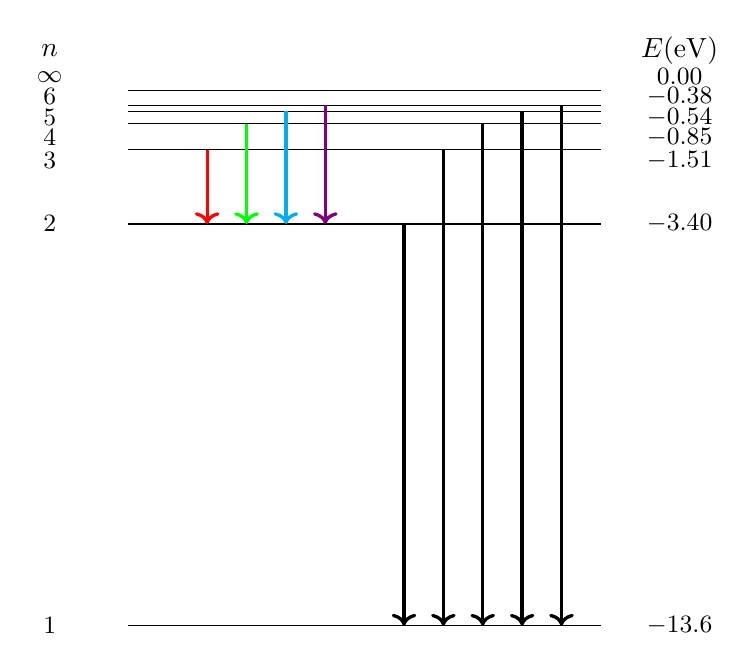
\begin{tikzpicture}
			\draw (1,0)--(7,0);
			\node at(0,0.5) {$ n $};
			\node at(8,0.5) {$ E(\mathrm{eV}) $};
			\draw (1,-6.8)--(7,-6.8);
			\draw (1,-1.7)--(7,-1.7);
			\draw (1,-0.755)--(7,-0.755);
			\draw (1,-0.425)--(7,-0.425);
			\draw (1,-0.27)--(7,-0.27);
			\draw (1,-0.19)--(7,-0.19);
			\node at(0,-0.08) {\small 6};
			\node at(8,-0.08) {\small $ -0.38 $};
			\node at(0,-0.35) {\small5};
			\node at(8,-0.35) {\small $ -0.54 $};
			\node at(0,0.17) {\small$\infty$};
			\node at(8,0.17) {\small 0.00};
			\node at(0,-0.6) {\small 4};
			\node at(8,-0.6) {\small $ -0.85 $};
			\node at(0,-0.9) {\small 3};
			\node at(8,-0.9) {\small $ -1.51 $};
			\node at(0,-1.7) {\small 2};
			\node at(8,-1.7) {\small $ -3.40 $};
			\node at(0,-6.8) {\small 1};
			\node at(8,-6.8) {\small $ -13.6 $};
			\draw [very thick,->,red] (2,-0.755)--(2,-1.7);
			\draw [very thick,->,green] (2.5,-0.425)--(2.5,-1.7);
			\draw [very thick,->,cyan] (3,-0.27)--(3,-1.7);
			\draw [very thick,->,violet] (3.5,-0.19)--(3.5,-1.7);
			\draw [very thick,->] (4.5,-1.7)--(4.5,-6.8);
			\draw [very thick,->] (5,-0.755)--(5,-6.8);
			\draw [very thick,->] (5.5,-0.425)--(5.5,-6.8);
			\draw [very thick,->] (6,-0.27)--(6,-6.8);
			\draw [very thick,->] (6.5,-0.19)--(6.5,-6.8);
		\end{tikzpicture}
		\caption{氢原子能级图}
	\end{figure}

	\subsection{测量样品的透过率}
	根据实验得到的谱线数据可作出如下图形(见下页):
	
	\begin{figure}[p]
		\centering
		\begin{tikzpicture}
			\begin{axis}[
				width=14cm,height=6cm,
				title={(a)\small 溴钨灯自身谱线(即基线)},
				xlabel=$ \lambda\;(\mathrm{nm}) $,
				ylabel=$ E\;(\mathrm{eV}) $,
				xmin=380,xmax=820,
				ymin=-50,ymax=650,
				xtick={400,450,500,550,600,650,700,750,800},
				ytick={0,100,200,300,400,500,600}
				]
				\addplot[thick,smooth,no marks] file {BrWu.txt};
			\end{axis}
		\end{tikzpicture}
	
		\begin{tikzpicture}
					\begin{axis}[
						width=14cm,height=6cm,
						legend pos=outer north east,
						title={\small (b)黑色滤波片的光透过率},
						xlabel=$ \lambda\;(\mathrm{nm}) $,
						ylabel=透过率(\%),
						xmin=380,xmax=820,
						ymin=0,ymax=100,
						xtick={400,450,500,550,600,650,700,750,800},
						ytick={0,20,40,60,80,100}
						]
						\addplot[thick,smooth,no marks] file {BWBlack.txt};
						%\addplot[thick,smooth,no marks,red] file {BWRed.txt};
						%\addplot[thick,smooth,no marks,green] file {BWGreen.txt};
						%\addplot[thick,smooth,no marks,blue] file {BWBlue.txt};
						%\addplot[thick,smooth,no marks,yellow] file {BWYellow.txt};
					\end{axis}
		\end{tikzpicture}
		
	\begin{tikzpicture}
		\begin{axis}[
			width=14cm,height=6cm,
			legend pos=outer north east,
			title={\small (c)红色滤波片的光透过率},
			xlabel=$ \lambda\;(\mathrm{nm}) $,
			ylabel=透过率(\%),
			xmin=380,xmax=820,
			ymin=0,ymax=100,
			xtick={400,450,500,550,600,650,700,750,800},
			ytick={0,20,40,60,80,100}
			]
			%\addplot[thick,smooth,no marks] file {BWBlack.txt};
			\addplot[thick,smooth,no marks,red] file {BWRed.txt};
			%\addplot[thick,smooth,no marks,green] file {BWGreen.txt};
			%\addplot[thick,smooth,no marks,blue] file {BWBlue.txt};
			%\addplot[thick,smooth,no marks,yellow] file {BWYellow.txt};
		\end{axis}
	\end{tikzpicture}
		
	\begin{tikzpicture}
		\begin{axis}[
			width=14cm,height=6cm,
			legend pos=outer north east,
			title={\small (d)绿色滤波片的光透过率},
			xlabel=$ \lambda\;(\mathrm{nm}) $,
			ylabel=透过率(\%),
			xmin=380,xmax=820,
			ymin=0,ymax=100,
			xtick={400,450,500,550,600,650,700,750,800},
			ytick={0,20,40,60,80,100}
			]
			%\addplot[thick,smooth,no marks] file {BWBlack.txt};
			%\addplot[thick,smooth,no marks,red] file {BWRed.txt};
			\addplot[thick,smooth,no marks,green] file {BWGreen.txt};
			%\addplot[thick,smooth,no marks,blue] file {BWBlue.txt};
			%\addplot[thick,smooth,no marks,yellow] file {BWYellow.txt};
		\end{axis}
	\end{tikzpicture}
	\end{figure}
	
	\newpage
	
	\begin{figure}[h]
		\centering
		\begin{tikzpicture}
			\begin{axis}[
				width=14cm,height=5cm,
				legend pos=outer north east,
				title={\small (e)蓝色滤波片的光透过率},
				xlabel=$ \lambda\;(\mathrm{nm}) $,
				ylabel=透过率(\%),
				xmin=380,xmax=820,
				ymin=0,ymax=100,
				xtick={400,450,500,550,600,650,700,750,800},
				ytick={0,20,40,60,80,100}
				]
				%\addplot[thick,smooth,no marks] file {BWBlack.txt};
				%\addplot[thick,smooth,no marks,red] file {BWRed.txt};
				%\addplot[thick,smooth,no marks,green] file {BWGreen.txt};
				\addplot[thick,smooth,no marks,blue] file {BWBlue.txt};
				%\addplot[thick,smooth,no marks,yellow] file {BWYellow.txt};
			\end{axis}
		\end{tikzpicture}
			
		\begin{tikzpicture}
			\begin{axis}[
				width=14cm,height=5cm,
				legend pos=outer north east,
				title={\small (f)黄色滤波片的光透过率},
				xlabel=$ \lambda\;(\mathrm{nm}) $,
				ylabel=透过率(\%),
				xmin=380,xmax=820,
				ymin=0,ymax=100,
				xtick={400,450,500,550,600,650,700,750,800},
				ytick={0,20,40,60,80,100}
				]
				%\addplot[thick,smooth,no marks] file {BWBlack.txt};
				%\addplot[thick,smooth,no marks,red] file {BWRed.txt};
				%\addplot[thick,smooth,no marks,green] file {BWGreen.txt};
				%\addplot[thick,smooth,no marks,blue] file {BWBlue.txt};
				\addplot[thick,smooth,no marks,yellow] file {BWYellow.txt};
			\end{axis}
		\end{tikzpicture}
		\caption{溴钨灯基线与不同颜色滤波片的光透过率曲线}
	\end{figure}
	
	根据$ A=-\lg T $可计算得到吸收系数图象为
	\begin{figure}[!h]
		\centering
		\includegraphics*[scale=0.5]{alpha.jpg}
		\caption{不同滤波片的吸收系数}
	\end{figure}
	
	\newpage
	
	\subsection{测量未知白光光源光谱}
	实验中分别测量LED灯白光(实际偏青色)、荣耀20闪光灯、小米6x闪光灯的光谱如下:
	\begin{figure}[h]
		\centering
		\begin{tikzpicture}
			\begin{axis}[
				width=14cm,height=6cm,
				xlabel=$ \lambda\;(\mathrm{nm}) $,
				ylabel=$ E\;(\mathrm{eV}) $,
				title={\small(a)LED灯白光},
				xmin=380,xmax=720,
				ymin=-50,ymax=400,
				xtick={400,450,500,550,600,650,700},
				ytick={0,100,200,300,400}
				]
				\addplot[thick,smooth,no marks] file {LED.txt};
			\end{axis}
		\end{tikzpicture}
		
		\begin{tikzpicture}
			\begin{axis}[
				width=14cm,height=6cm,
				xlabel=$ \lambda\;(\mathrm{nm}) $,
				ylabel=$ E\;(\mathrm{eV}) $,
				title={\small(b)荣耀20闪光灯},
				xmin=380,xmax=720,
				ymin=-50,ymax=700,
				xtick={400,450,500,550,600,650,700},
				ytick={0,100,200,300,400,500,600,700}
				]
				\addplot[thick,smooth,no marks] file {Honor20.txt};
			\end{axis}
		\end{tikzpicture}
		
		\begin{tikzpicture}
			\begin{axis}[
				width=14cm,height=6cm,
				xlabel=$ \lambda\;(\mathrm{nm}) $,
				ylabel=$ E\;(\mathrm{eV}) $,
				title={\small(c)小米6x闪光灯},
				xmin=380,xmax=720,
				ymin=-50,ymax=500,
				xtick={400,450,500,550,600,650,700},
				ytick={0,100,200,300,400,500}
				]
				\addplot[thick,smooth,no marks] file {Mi6x.txt};
			\end{axis}
		\end{tikzpicture}
		\caption{未知白光光源的光谱}
	\end{figure}

	由上图可以看出实验室提供的LED灯白光视觉上偏青色的原因是在光谱中缺失了红光波段,而两个型号手机的闪光灯白光构成相似。
	
	\newpage
	\section{实验总结}
	\subsection{思考题}
	1.测量中对出射和入射狭缝的宽度有什么要求?
	
	\textit{根据理论推导可知谱线的宽度与出入射狭缝的宽度均成正比。故而为了得到更高质量的谱线,需适当减小出入射狭缝的宽度提高分辨率。但若狭缝过窄,入射的光强过小,既有可能无法测得数据,也可能因能量过小而遭到干扰加大误差。实际实验中通常不调节出射缝宽,仅通过调节入射缝宽以得到既能保证测量也能保证一定分辨率的光谱。}
	
	~\
	
	2.光谱仪的入射狭缝除了通光作用,与分辨率的关系是什么?
	
	\textit{根据实验原理部分可知:入射狭缝越窄,分辨率越高。}
	
	~\
	
	3.光栅光谱仪的分辨极限是由什么条件决定?
	
	\textit{记$ N $为光栅使用面积的刻线总数目,$ k $为衍射级,故而光栅光谱仪的理论分辨极限为$ kN $。实际使用中,分辨率还会受到狭缝宽度、光路系统灯因素的影响。}
	
	~\
	
	4.什么是光栅的谱级重叠?如何消除?
	
	\textit{根据光栅方程}
	\[m\lambda=d(\sin\alpha\pm\sin\beta)\]
	\textit{可知谱级与波长满足$ m_1\lambda_1=m_2\lambda_2=m_3\lambda_3=\cdots $的各级光谱线具有同样的衍射角,会在焦面的同一位置上出现,这就是光谱的谱级重叠现象。通常可以用相应波段的滤光片滤掉无用的波段。}
	
	~\
	
	5.光源的位置不同会对谱图有什么影响?
	
	\textit{光源的位置不同会影响入射的光强,体现在谱线上即为纵坐标的大小。但改变光源位置不会对谱线位置等实验结果造成较大影响。}
	
	~\
	
	6.测量到的谱线都有一定的宽度是什么原因?
	
	\textit{仪器实际测得的谱线轮廓,是在谱线自身轮廓、光源轮廓等多个因素下影响作用得到的结果。此外实验并非在真空中进行,在光路系统中也存在一定损耗,即便原波长离散,最后仍会有一定宽度。}
	
	\newpage
	
	\subsection{心得体会与反思收获}
	在本次实验中,使用计算机软件配合光栅光谱仪进行相关操作,进一步体会了现代实验中的便利性。得益于计算机与自动化产业的发展,实验者在实验中所需要做的工作得到了大大简化,不需要对光学器件进行精密的调节、为读数与精度焦头烂额,这些工作都已交由计算机代为实现。当然,实验中仍会出现各种问题与需求,解决问题、满足需求都是计算机无能为力的工作,这时候实验者的实验素养与物理知识就起到了重要作用。比如,在对未知白光的光谱测定实验中,由于缺乏合适的支架,无论是实验室提供的LED灯还是自己与同学的手机,都让我在寻找并固定于合适的位置这些过程中耗费了不少精力。
\end{document}